\chapter{Serie di Fourier}
\section{Serie di Fourier nel continuo}
Le serie di Fourier si basano sulle \textbf{funzioni perioche}, ovvero funzioni che
si ripetono ad intervalli regolari.
\begin{definizione}[\textbf{Funzione periodica}]
    Una funzione $f:\mathbb{R}\to \mathbb{R}$ si dice \textbf{periodica} se
    $\forall x\in \mathbb{R}, \exists T \in \mathbb{R}$ tale che:
    \begin{equation}
        f(x+n \cdot T) = f(x) \quad \forall n \in \mathbb{Z} \text{ e } \forall x \in \mathbb{R}
    \end{equation}
\end{definizione}
\begin{proposizione}
    Se una funzione periodica di periodo $p$ è notata in un generico intervallo
    di ampiezza $p$ allora è nota ovunque.
\end{proposizione}
Il risultato precedente sarà estremamente utile. Infatti, ci permette di ricondurre
lo studio/analisi di una funzione periodica di periodo $p$ solamente nell'intervallo
$[0, p]$.
\begin{proposizione}
    L'integrale su un intervallo di ampiezza $p$ di una funzione periodica $f$
    di periodo $p$ non dipende dagli estremi di integrazione.
    \begin{equation}
        \int_{a}^{a + p}f(t)dt = \int_{b}^{b + p}f(t)dt \quad \forall a,b
    \end{equation}
    \begin{proof}
        Significa dimostrare la seguente uguaglianza:
        \begin{equation*}
            \int_{a}^{a + p}f(t)dt = \int_{0}^{p}f(t)dt
        \end{equation*}
        Per le proprietà degli integrali sappiamo che:
        \begin{equation*}
            \int_{a}^{a+p}f(t)dt =  \int_{a}^{p}f(t)dt + \int_{p}^{a+p}f(t)dt =
            \int_{a}^{0}f(t)dt +\int_{0}^{p}f(t)dt+ \int_{p}^{a+p}f(t)dt
        \end{equation*}
        Utilizzando il metodo di sostituzione, introduciamo $s = t - p$, di conseguenza
        $t= p \iff s=0$ e $t = p + a \iff s = a$. Per concludere la sostituzione
        dobbiamo aggiornare i differenziali e gli estremi di integrazione.
        Per i differenziali avremo $ds = dt$ perché $\frac{\partial s}{\partial s} = 1$
        e $\frac{\partial t-p}{\partial t} = 1$.

        Quindi gli integrali diventano
        \begin{equation*}
            \int_{a}^{0}f(t)dt +\int_{0}^{p}f(t)dt+ \int_{p}^{a+p}f(t)dt =
            \int_{a}^{0}f(t)dt +\int_{0}^{p}f(t)dt+ \int_{0}^{a}f(s)ds =
        \end{equation*}

        Ma essendo $f$ periodica di periodo $p$, sapendo che $s = t + p$ e $p$ è
        il periodo allora $f(s) = f(t)$, quindi $\int_{0}^{a}f(s)ds = \int_{0}^{a}f(t)dt$,
        perciò:
        \begin{equation*}
            \begin{aligned}
                \int_{a}^{0}f(t)dt + \int_{0}^{p}f(t)dt + \int_{0}^{a}f(s)ds =
                \int_{a}^{0}f(t)dt + \int_{0}^{p}f(t)dt + \int_{0}^{a}f(t)dt = \\
                -\int_{0}^{a}f(t)dt + \int_{0}^{a}f(t)dt + \int_{0}^{p}f(t)dt =
                \int_{0}^{p}f(t)dt
            \end{aligned}
        \end{equation*}
    \end{proof}
\end{proposizione}
\begin{nota}
    Nei computer, la rappresentazione di un integrale viene approssimata nel
    seguente modo:
    \begin{equation*}
        \int_{0}^{p}f(t)dt \approx \sum_{i=1}^{x_n}\omega_i f(t_i)
    \end{equation*}
\end{nota}
Il nostro obiettivo è quello di modificare una funzione periodica in modo da
rendere più gestibile la periodicità. Consideriamo una funzione periodica di
di periodo $t$ e la vogliamo trasformare in una funzione periodica di un generico
periodo $p$.

Per ottenere questo risultato possiamo modificare l'argomento della funzione
periodica nel seguente modo:
\begin{equation}
    f(t) = f\left(\frac{t}{p}\right)
\end{equation}
Così facendo, se $p < t$ allora stiamo accorciando il periodo della funzione. Al
contrario, se $p > t$ stiamo allungando il periodo della funzione.
\begin{proof}
    Per dimostrarlo possiamo prendere una funzione periodica generica $f$ di
    periodo $t$ e posso testare che $f(x) = f\left( n \cdot \frac{t}{p} + x\right)$
    sia periodica di periodo $p$, ovvero che $f(x + np) = f(x) \iff
        f\left(\frac{t}{p}x + np\right) = f(\frac{t}{p}x)$.

    \begin{equation*}
        f\left(x + n \cdot p\right) = f\left(\frac{t}{p}\cdot (x + np)\right) =
        f\left(\frac{tx}{p} + \frac{tnp}{p}\right) = f\left(\frac{tx}{p} + nt\right)
        = f\left(\frac{tx}{p}\right) = f'(x)
    \end{equation*}
    perché $f$ è periodica di periodo $t$.
\end{proof}

Utilizzeremo per lo più le seguenti funzioni $\sin\left(\frac{2\pi k}{p}t\right)$
e $\cos \left(\frac{2\pi k}{p}t\right)$. Dove $k$ è un intero positivo che permette
di alterare la frequenza della funzione.
\begin{proposizione}\label{prop:integrali_sinusoidi}
    Per ogni $k \geq 1$ vale il seguente integrale:
    \begin{equation*}
        \int_{0}^{p}\sin \left(\frac{2\pi k}{p}t\right) dt =
        \int_{0}^{p}\cos \left(\frac{2\pi k}{p}t\right) dt = 0
    \end{equation*}
    \begin{proof}
        Possiamo risolvere i singoli integrali, per esempio con la sostituzione
        introduciamo la variabile $s= \frac{2\pi k}{p}t$ quindi $\frac{p}{2\pi k}ds =dt$
        allora:
        \begin{equation*}
            \int_{0}^{p}\sin \left(\frac{2\pi k}{p}t\right) dt =
            \int_{0}^{2k\pi}\sin \left(s\right)\frac{p}{2\pi k}ds =
            \frac{p}{2\pi k} \int_{0}^{2k\pi}\sin \left(s\right)ds =
            \frac{p}{2\pi k} \left[-cos(s)\right]_0^{2k\pi} = 0
        \end{equation*}
        Lo stesso ragionamento può essere applicato al coseno.
    \end{proof}
\end{proposizione}
\begin{proposizione}
    Presa una qualsiasi coppia di valori interi $l, k > 0$ vale il seguente integrale:
    \begin{equation}
        \int_{0}^{p}\sin\left(\frac{2\pi l}{p}t\right) \cdot \cos\left(\frac{2\pi k}{p}t\right) dt = 0
    \end{equation}
    \begin{proof}
        Risolviamolo con la sostituzione $s= \frac{2\pi t}{p}$ quindi $ds = \frac{p}{2\pi}dt$.
        \begin{equation*}
            \int_{0}^{p}\sin\left(\frac{2\pi l}{p}t\right)\cdot \cos\left(\frac{2\pi k}{p}t\right) dt =
            \int_{0}^{2\pi}\sin\left(ls\right)\cdot \cos\left(ks\right)\frac{p}{2\pi} ds =
            \frac{p}{2\pi}\int_{0}^{2\pi}\sin\left(ls\right)\cdot \cos\left(ks\right) ds
        \end{equation*}
        Utilizzando la relazione $\frac{1}{2}\left(\sin(\alpha +\beta) +
            \sin(\alpha-\beta)\right) = \sin\left(\alpha\right)\cos\left(\beta\right)$
        possiamo dire:
        \begin{equation*}
            \begin{aligned}
                \frac{p}{2\pi}\int_{0}^{2\pi}\sin\left(ls\right)\cdot \cos\left(ks\right) ds =
                \frac{p}{2\pi}\frac{1}{2}\int_{0}^{2\pi}\sin\left((l+k)s\right)+ \sin\left((l-k)s\right) ds= \\
                =\frac{p}{4\pi}\left(\int_{0}^{2\pi}\sin\left((l+k)s\right)ds + \int_{0}^{2\pi}\sin\left((l-k)s\right) ds\right)=0
            \end{aligned}
        \end{equation*}
        Si annullano perché coincide con l'integrale della nota precedente.
    \end{proof}
\end{proposizione}
\begin{proposizione}
    Presa una qualsiasi coppia di valori interi $l, k > 0$ vale il seguente integrale:
    \begin{equation*}
        \int_{0}^{p}\cos\left(\frac{2\pi l}{p}t\right) \cdot
        \cos\left(\frac{2\pi k}{p}t\right) dt = \begin{cases}
            \frac{p}{2} & k=l      \\
            0           & k \neq l \\
        \end{cases}
    \end{equation*}
    l'integrale tra il prodotto dei coseni con frequenza diversa allora il risultato
    è nullo.
    \begin{proof}
        Per dimostralo usiamo sempre la sostituzione $s=\frac{2\pi}{p}dt$ e $\frac{p}{2\pi}ds = dt$.
        Sostituendo otteniamo:
        \begin{equation*}
            \frac{p}{2\pi}\int_{0}^{2\pi} \cos(ks) \cdot \cos(ls) ds
        \end{equation*}
        Utilizzando un procedimento simile a quello di prima, possiamo scrivere:
        \begin{equation*}
            \frac{1}{2} (\cos(\alpha + \beta) + \cos(\alpha - \beta)) = \cos(\alpha)\cos(\beta)
        \end{equation*}
        Quindi:
        \begin{equation*}
            \frac{p}{2\pi}\int_{0}^{2\pi} \cos(ks) \cdot \cos(ls) ds =
            =\frac{p}{2\pi}\int_{0}^{2\pi} \frac{1}{2}\cos((k+l)s) +\cos((k-l)s) ds =
            \frac{p}{4\pi}\int_{0}^{2\pi}\cos((k+l)s) +\cos((k-l)s) ds
        \end{equation*}
        Per il caso $k \neq l$ allora otteniamo l'integrale della proposizione
        \ref{prop:integrali_sinusoidi} e quindi è uguale a $0$.
        Se $k = l$ allora $\int_{0}^{2\pi} \cos(2k s) ds = 0$ mentre
        $\int_{0}^{2\pi}cos(0s)ds = s|_{0}^{2\pi} = 2\pi$ il quale deve essere
        moltiplicato per $\frac{p}{4\pi}$ che era il coefficiente davanti all'integrale.

        Quindi se $k=l$ allora l'integrale vale $\frac{p}{2}$.
    \end{proof}
\end{proposizione}
Per il caso $\sin \cdot \sin$ si ottiene un risultato analogo al caso $\cos \cdot \cos$
modificando solamente la seguente relazione:
\begin{equation*}
    \frac{1}{2} (\cos(\alpha + \beta) + \cos(\alpha - \beta)) = \cos(\alpha)\cos(\beta) \to
    \frac{1}{2} (\cos(\alpha - \beta) - \cos(\alpha + \beta)) = \sin(\alpha)\sin(\beta)
\end{equation*}

La stessa dimostrazione si può effettuare per il caso $\sin \cdot \sin$
\begin{equation}
    \int_{0}^{p}\sin \left(\frac{2\pi}{p} kt\right) \sin \left(\frac{2\pi}{p} lt
    \right) dt = \begin{cases}
        \frac{p}{2} & l = k      \\
        0           & altrimenti
    \end{cases}
\end{equation}

L'idea alla basa della serie di Fourier è quella di scrivere una generica funzione
periodica $f:\mathbb{R}\to \mathbb{R}$ di periodo $p$ in una combinazione di $\sin$
e $\cos$.
\begin{definizione}[\textbf{Serie di Fourier}]
    Sia $f:\mathbb{R}\to \mathbb{R}$ una funzione periodica di periodo $p$.
    \begin{equation}
        f(t) = a_0 + \sum_{k=1}^{\infty} \left[a_k \cos (\frac{2\pi}{p}kt) +
            \beta_k \sin(\frac{2\pi}{p} kt)\right]
    \end{equation}
\end{definizione}

L'uguaglianza precedente è lecita perché specifica che una funzione periodica di
periodo $p$ può essere riscritta come combinazioni lineari di funzioni periodiche,
anche esse di periodo $p$. Importante è anche la limitazione della sommatoria a
$\infty$ perché significa una funzione è combinazione lineare di \textbf{tutte}
le funzioni periodiche.

All'atto pratico la sommatoria infinita è impossibile da calcolare, quindi si
approssima la funzione ad un $N$ molto grande.

In aggiunta si può notare che i coefficienti $a_0, a_1, \dots$ partono dall'indice
$0$ mentre $b_1,b_2,\dots$ partono dall'indice $1$. Questo è dato dal fatto che
quando $k = 0$ si ha:
\begin{equation*}
    a_0\cos (\frac{2\pi}{p}0t) +\beta_0\sin(\frac{2\pi}{p}0t) = a_0\cdot 1 + b_0
    \cdot 0 = a_0
\end{equation*}

Per utilizzare questa approssimazione mediante la serie, dobbiamo calcolare
facilmente e velocemente i coefficienti $a_i,b_i$.

Calcoliamo per prima cosa $a_0$, per ipotesi sappiamo che l'uguaglianza che esprime
la serie di Fourier è valida, allora anche gli integrali delle due parti saranno
uguali.
\begin{equation*}
    \int_{0}^{p}f(t) dt=\int_{0}^{p} a_0 + \sum_{k=1}^{\infty}\left[a_k\cos
        (\frac{2\pi}{p}kt) +\beta_k\sin(\frac{2\pi}{p}kt)\right]dt
\end{equation*}
Applicando le proprietà degli integrali si ottiene:
\begin{equation*}
    \int_{0}^{p}f(t) dt=a_0\int_{0}^{p} 1dt + \sum_{k=1}^{\infty}\left[a_k
        \int_{0}^{p}\cos (\frac{2\pi}{p}kt)dk +\beta_k\int_{0}^{p}\sin(
        \frac{2\pi}{p}kt)dt\right]
\end{equation*}
Grazie alle dimostrazioni effettuate precedentemente sappiamo che:
\begin{equation*}
    \int_{0}^{p}\sin \left(\frac{2\pi k}{p}t\right) dt =
    \int_{0}^{p}\cos \left(\frac{2\pi k}{p}t\right) dt = 0
\end{equation*}
di conseguenza abbiamo che gli integrali presenti nella sommatoria si annullano,
otteniamo quindi:
\begin{equation*}
    \int_{0}^{p}f(t) dt = a_0\int_{0}^{p} 1dt  = a_0p\implies a_0 = \frac{1}{p}
    \int_{0}^{p}f(t) dt
\end{equation*}
Questa espressione si può calcolare perché $f$ è sempre nota.
\begin{nota}
    La seguente espressione è chiamata anche media integrale nell'intervallo $[0,p]$.
    \begin{equation*}
        a_0 = \frac{1}{p}\int_{0}^{p}f(t) dt
    \end{equation*}
\end{nota}
Per calcolare i coefficienti $a_k$ possiamo moltiplicare entrambe le parti
dell'uguaglianza per $\cos\left(\frac{2\pi}{p}kt\right)$ e successivamente
integrare. In questo modo otteniamo:
\begin{equation*}
    \begin{aligned}
        \int_{0}^{p}f(t) \cdot \cos\left(\frac{2\pi}{p}kt\right) dt = \\ a_0\int_{0}^{p}
        \cos\left(\frac{2\pi}{p}kt\right) dt + \sum_{j=1}^{\infty}\left[a_j\int_{0}^{p}
            \cos \left(\frac{2\pi}{p}jt\right) \cos\left(\frac{2\pi}{p}kt\right)dk +
            \beta_j\int_{0}^{p}\sin\left(\frac{2\pi}{p}jt\right)\cos\left(\frac{2\pi}{p}kt\right)dt\right]
    \end{aligned}
\end{equation*}
Sfruttando le proposizioni definite in precedenza possiamo affermare che:
\begin{equation*}
    \begin{array}{c}
        a_0\int_{0}^{p}\cos \left(\frac{2\pi}{p}kt\right)dt = 0 \\
        \beta_j\int_{0}^{p}\sin\left(\frac{2\pi}{p}jt\right)\cos \left(\frac{2\pi}{p}kt\right)dt=0
    \end{array}
\end{equation*}
perciò, otteniamo:
\begin{equation*}
    \int_{0}^{p}f(t)\cos \left(\frac{2\pi}{p}kt\right) dt = \sum_{j=1}^{\infty}
    \left[a_j\int_{0}^{p}\cos \left(\frac{2\pi}{p}jt\right)\cos \left(
        \frac{2\pi}{p}kt\right)dk \right]
\end{equation*}
Per le proposizioni che abbiamo in precedenza, sappiamo che l'integrale del prodotto
di due coseni con frequenza diversa è nullo. Quindi rimane solamente il caso in
cui le frequenze sono uguali, ovvero $j=k$. Questo cui permette di ottenere:
\begin{equation*}
    \int_{0}^{p}f(t)\cos \left(\frac{2\pi}{p}kt\right) dt = a_k\int_{0}^{p}\cos
    \left(\frac{2\pi}{p}kt\right)\cos \left(\frac{2\pi}{p}kt\right)dk = a_k \frac{p}{2}
    \iff a_k =\frac{2}{p}  \int_{0}^{p}f(t)\cos \left(\frac{2\pi}{p}kt\right) dt
\end{equation*}
Il conto di $a_k$ è indipendente dagli altri valori di $a_j$ e quindi può essere
calcolato indipendentemente dagli altri coefficienti.

Successivamente dobbiamo calcolare i coefficienti $b_k$, la metodologia è la stessa
degli $a_k$ solo che in questo caso la funzione per cui moltiplichiamo entrambi
i membri è:
\begin{equation*}
    \sin\left(\frac{2\pi}{p}kt\right)
\end{equation*}
\begin{equation*}
    \begin{array}{l}
        \int_{0}^{p}f(t)\sin\left(\frac{2\pi}{p}kt\right) dt = \\
        = a_0 \int_{0}^{p} \sin\left(\frac{2\pi}{p}kt\right) dt + \sum_{j=1}^{\infty}
        \left[a_j\int_{0}^{p}\cos \left(\frac{2\pi}{p}jt\right)\sin\left(\frac{2\pi}{p}kt\right)dk
            + \beta_j \int_{0}^{p}\sin\left(\frac{2\pi}{p}jt\right)\sin\left(\frac{2\pi}{p}kt
            \right)dt\right]
    \end{array}
\end{equation*}
Grazie alle proposizioni definite in precedenza possiamo affermare che:
\begin{equation*}
    \begin{array}{c}
        a_0\int_{0}^{p}\sin \left(\frac{2\pi}{p}kt\right)dt = 0 \\
        a_j\int_{0}^{p}\cos\left(\frac{2\pi}{p}jt\right)\sin \left(\frac{2\pi}{p}kt\right)dt=0
    \end{array}
\end{equation*}
perciò, otteniamo:
\begin{equation*}
    \int_{0}^{p}f(t)\sin \left(\frac{2\pi}{p}kt\right) dt = \sum_{j=1}^{\infty}
    \left[\beta_j\int_{0}^{p}\sin \left(\frac{2\pi}{p}jt\right)\sin \left(
        \frac{2\pi}{p}kt\right)dk \right]
\end{equation*}
Per le proposizioni che abbiamo in precedenza, sappiamo che l'integrale del prodotto
di due seni con frequenza diversa è nullo. Quindi rimane solamente il caso in
cui le frequenze sono uguali, ovvero $j=k$. Questo cui permette di ottenere:
\begin{equation*}
    \int_{0}^{p}f(t)\sin \left(\frac{2\pi}{p}kt\right) dt = \beta_k\int_{0}^{p}\sin
    \left(\frac{2\pi}{p}kt\right)\sin \left(\frac{2\pi}{p}kt\right)dk = \beta_k \frac{p}{2}
    \iff \beta_k =\frac{2}{p}  \int_{0}^{p}f(t)\sin \left(\frac{2\pi}{p}kt\right) dt
\end{equation*}

\begin{definizione}[\textbf{Funzione pari}]
    Una funzione $f:\mathbb{R}\to \mathbb{R}$ si dice \textbf{pari} se:
    \begin{equation}
        f(t) = f(-t) \quad \forall t \in \mathbb{R}
    \end{equation}
\end{definizione}
\begin{definizione}[\textbf{Funzione dispari}]
    Una funzione $f:\mathbb{R}\to \mathbb{R}$ si dice \textbf{dispari} se:
    \begin{equation}
        f(t) = -f(-t) \quad \forall t \in \mathbb{R}
    \end{equation}
\end{definizione}
Sapendo che la funzione $\sin$ è dispari e la funzione $\cos$ è pari, possiamo
dire che se $f$ è pari allora i coefficienti $\beta_i = 0$ mentre se $f$ è dispari
allora i coefficienti $a_i = 0$.
\begin{proposizione}
    Prese due funzioni $f,g:\mathbb{R}\to \mathbb{R}$ tali per cui $f$ è pari e
    $g$ è dispari allora $h(x)=f(x)g(x)$ è dispari
    \begin{proof}
        Se $f(x)$ è pari se e solo se $f(x) = f(-x),\forall x\in \mathbb{R}$.
        Se $g(x)$ è dispari se e solo se $g(x) = -g(-x),\forall x\in \mathbb{R}$.
        Quindi per dimostrare $h(x)$ dispari allora possiamo partire dalla definizione.
        \begin{equation*}
            h(x) = f(x)g(x) = f(-x) (-g(-x)) = - f(-x)g(-x) = -h(-x)
        \end{equation*}
        Quindi abbiamo dimostrato che $h$ è dispari.
    \end{proof}
\end{proposizione}
Ricorda che la periodicità delle funzioni viene mantenuta.
\begin{proposizione}
    Presa una funzione $f:\mathbb{R}\to \mathbb{R}$ dispari e un intervallo simmetrico
    rispetto all'origine $[-a,a]$ con $a>0$ allora:
    \begin{equation}
        \int_{-a}^{a} f(x)dx = 0
    \end{equation}
    \begin{proof}
        Per dimostrare questa proposizione ci basiamo sul fatto che:
        \begin{equation*}
            \int_{-a}^{a} f(x)dx = \int_{-a}^{0} f(x)dx + \int_{0}^{a} f(x)dx =
            -\int_{0}^{-a} f(x) dx+ \int_{0}^{a} f(x)dx
        \end{equation*}
        Dato che $f$ è dispari allora $ \int_{0}^{-a} f(x) = \int_{0}^{a} f(x)$
        e quindi:
        \begin{equation*}
            -\int_{0}^{a} f(x) dx + \int_{0}^{a} f(x) dx = 0
        \end{equation*}
    \end{proof}
\end{proposizione}
Sfruttando i risultati delle due proposizioni appena presentate, possiamo dire che
se $f$ è una funzione dispari possiamo verificare che $a_k = 0, \, \forall k \ge 0$.
\begin{equation*}
    a_k = \int_{0}^{p} f(t) \cos\left(\frac{2 \pi}{p} kt\right) dt =
    \int_{-\frac{p}{2}}^{\frac{p}{2}} f(t) \cos\left(\frac{2 \pi}{p} kt\right) dt =
    \int_{-\frac{p}{2}}^{\frac{p}{2}} H(x) dx = 0
\end{equation*}
sapendo che $H(x)$ è dispari in quanto sto moltiplicando una funzione pari con una
funzione dispari. Nel caso specifico di $a_0$ ho che:
\begin{equation*}
    a_0 =\frac{1}{p} \int_{0}^{p}f(x)dx = \frac{1}{p} \int_{-\frac{p}{2}}^{\frac{p}{2}}f(x)dx = 0
\end{equation*}
In modo analogo si procede nel caso in cui $f$ è pari:
\begin{equation*}
    b_k = \int_{0}^{p} f(t) \sin\left(\frac{2 \pi}{p} kt\right) dt =
    \int_{-\frac{p}{2}}^{\frac{p}{2}} f(t) \sin\left(\frac{2 \pi}{p} kt\right) dt =
    \int_{-\frac{p}{2}}^{\frac{p}{2}} G(x) dx = 0
\end{equation*}
sapendo che $G(x)$ è dispari in quanto sto moltiplicando una funzione pari con una
funzione dispari.
\begin{nota}
    Posso cambiare l'intervallo di integrazione e passare da $[0,p]$ a $[-\frac{p}{2},\frac{p}{2}]$
    in quanto le funzioni sono periodiche di periodo $p$.
\end{nota}

Riassumendo, per calcolare la trasformata di Fourier $f(x)$ allora ci serve:
\begin{itemize}
    \item Essere certi che $f(x)$ sia periodica.
    \item Dobbiamo calcolare $\alpha_k$ e $\beta_k$, quindi devono esistere
          ed essere finiti i seguenti integrali.
          \begin{equation*}
              a_k = \frac{2}{p}\int_{0}^{p}f(x)\cos\left(\frac{2\pi k}{p}x\right)
              dx \quad \beta_k=\frac{2}{p}\int_{0}^{p}f(x)\sin\left(\frac{2\pi k}{p}x\right)dx
          \end{equation*}
          dal momento che $\cos$ e $\sin$ sono sempre integrabili allora i vincoli
          sono solo su $f$.
\end{itemize}
\begin{nota}
    Possiamo rappresentare la trasformata di Fourier per quelle funzioni che hanno
    un numero finito di discontinuità di tipo salto.
\end{nota}

La convergenza della serie di Fourier dipende dalla regolarità delle funzioni $f$,
infatti se ci sono delle discontinuità di tipo salto allora si hanno delle
convergenze meno precise. Si hanno i fenomeni di \textbf{Gibbs} ovvero si hanno andamenti
oscillatori vicino al punto di discontinuità, questi sono dovuti dal fatto che si
stanno approssimando dei punti di discontinuità di tipo salto con funzioni che non
li hanno.

convergenze meno precise. Si hanno i fenomeni di \textbf{Gibbs} ovvero si hanno andamenti
oscillatori vicino al punto di discontinuità, questi sono dovuti dal fatto che si
stanno approssimando dei punti di discontinuità di tipo salto con funzioni che non
li hanno.

Per risolvere questo problema possiamo introdurre nella sommatoria delle funzioni
che avranno gli stessi punti di discontinuità negli stessi valori.

\begin{teorema}[\textbf{Convergenza della serie di Fourier}]
    Sia $f:\mathbb{R}\to \mathbb{R}$ periodica, assumiamo che $f$ sia $C^1$ (continua
    fino alla prima derivata) a tratti allora se $f$ è continua in $t \in \mathbb{R}$
    fino alla prima derivata) a tratti allora se $f$ è continua in $t \in \mathbb{R}$
    la serie $f_N$ converge a $f(t)$, altrimenti se non è continua allora $f_N$
    converge a:
    \begin{equation*}
        \frac{\lim_{x\to t^-}f(x) +\lim_{x\to t^+}f(x)}{2}
    \end{equation*}
\end{teorema}
La serie converge alla media dei due limiti se $f$ non è continua, però prima e
dopo si ha fenomeni di Gibbs, però più incrementiamo il valore di $N$ maggiore
sarà la traslazione del movimento verso il punto di discontinuità.

Più precisamente la convergenza della serie dipende da come è fatta $f$:
\begin{itemize}
    \item Se $f$ è regolare la serie converge.
    \item Se $f$ presenta una discontinuità sulla derivata prima, allora nel
          punto in cui è presente tale discontinuità la convergenza sarà lenta.
    \item Se $f$ ha un punto di discontinuità di tipo salto, allora la serie
          converge alla media dei limiti nel punto con la conseguente presenza
          del fenomeno di GIBBS.
\end{itemize}
\subsection{Serie di Fourier per funzioni non periodiche}
Per ora abbiamo visto solo l'utilizzo della serie di Fourier per il caso di funzioni
$f$ periodiche di periodo $p$ e analizzandole nell'intervallo $[0,p]$. In realtà
possiamo generalizzare il ragionamento fatto finora per estendere la serie di Fourier
a una generica funzione $g(x)$ in un generico intervallo $[a,b]$.

Facendo opportuni cambi di variabili, anziché considerare un generico intervallo
$[a, b]$, si può sempre pensare che la funzione $f$ sia definita nell'intervallo
$[0, p]$. Questo può essere fatto utilizzando la seguente trasformazione:
\begin{equation}
    x = \frac{b - a}{p} x' + a \quad x' \in [0, p] \implies x \in [a, b]
\end{equation}

In questo modo si riesce a portare la funzione nell'intervallo canonico definendo:
\begin{equation*}
    \stackrel{\sim}{g}(x) = g\left(\frac{b-a}{p}x'+a\right), \quad \forall x' \in [a,b], x \in [0,p]
\end{equation*}
Si apre ora la questione di come creare una funzione periodica a partire da questa
funzione $\stackrel{\sim}{g}(x)$ definita nell'intervallo $[0, p]$. Un primo
tentativo potrebbe essere quello di periodizzarla per ripetizione.
tentativo potrebbe essere quello di periodizzarla per ripetizione.
\begin{figure}[!ht]
    \centering
    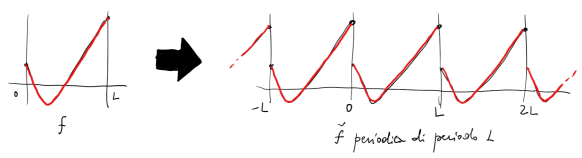
\includegraphics[width=0.5\textwidth]{img/Serie/ripetizione.png}
    \caption{Periodizzazione della funzione $\stackrel{\sim}{g}(x)$}
    \label{fig:ripetizione}
\end{figure}

Agendo in questo modo abbiamo creato delle discontinuità sulla funzione. Di conseguenza
l'approssimazione data dalle serie di Fourier sarà soggetta al fenomeno di Gibbs.

In realtà $\stackrel{\sim}{g}(x)$ in un modo più intelligente risolvendo eventuali
discontinuità di salto, ovvero presa $\stackrel{\sim}{g}(x)$, la si porta in $[0,p]$,
si specchia la funzione rispetto l'asse delle $y$ e poi replichiamo la funzione
infinite volte, ottenendo una funzione periodica di periodo $2p$.
\begin{figure}[!ht]
    \centering
    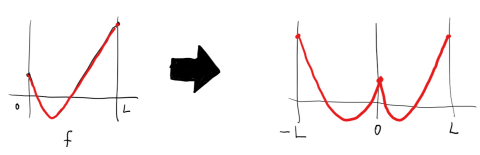
\includegraphics[width=0.5\textwidth]{img/Serie/specchio.png}
    \caption{Periodizzazione della funzione $\stackrel{\sim}{g}(x)$}
    \label{fig:specchio}
\end{figure}

Utilizzando quest'ultimo la trasformazione di Fourier si chiamerà \textbf{cosine trasformation},
perché $\stackrel{\sim}{g}(x)$ sarà pari e quindi la sua approssimazione sarà
composta solamente dai coefficienti del coseno.

Avendo definito la funzione $\stackrel{\sim}{g}(x)$ per renderla periodica, il
calcolo della trasformata di Fourier si complicherà, in quanto viene chiesto di
calcolare i coefficienti nell'intervallo di periodicità $[0, 2L]$.

Possiamo semplificarci la vita sfruttando la funzione iniziale nell'intervallo
$[a,b]$, sapendo che $\stackrel{\sim}{g}(x)$ coincide con quella di partenza
specchiata rispetto l'asse $y$ e poi resa periodica, abbiamo quindi costruito una
funzione pari.

Vediamo ora come possiamo calcolare i coefficienti della serie di Fourier per
questa funzione $\stackrel{\sim}{g}(x)$.

Iniziamo con il calcolo del coefficiente $a_0$:
\begin{equation}
    a_0 = \frac{1}{2L} \int_{0}^{2L} \stackrel{\sim}{g}(s)ds = \frac{1}{2L}
    \int_{-L}^{L} \stackrel{\sim}{g}(s)ds = \frac{1}{2L} 2 \int_{0}^{L} \stackrel{\sim}{g}(s)ds
    = \frac{1}{L} \int_{0}^{L} g(s)ds = \frac{1}{L} \int_{0}^{L} g\left(\frac{b - a}{L} s + a\right)ds
\end{equation}
Nello specifico, essendo la funzione periodica e pari, possiamo fare le seguenti
considerazioni:
\begin{itemize}
    \item Portare gli integrali dall'intervallo $[0,2L]$ all'intervallo $[-L,L]$
    \item Semplificare il calcolo di $2\int_{0}^{L}$ che coincide con la funzione iniziale
\end{itemize}
Per quanto riguarda il calcolo del generico coefficiente $a_k$:
\begin{equation}
    \begin{array}{l}
        a_k = \frac{2}{2L} \int_{0}^{2L} \stackrel{\sim}{g}(s) \cos\left(\frac{2\pi k}{2L}s\right)ds
        = \frac{1}{L} \int_{0}^{2L} \stackrel{\sim}{g}(s) \cos\left(\frac{\pi k}{L}s\right)ds \\
        = \frac{1}{L} \int_{-L}^{L} \stackrel{\sim}{g}(s) \cos\left(\frac{\pi k}{L}s\right)ds
        = \frac{2}{L} \int_{0}^{L} \stackrel{\sim}{g}(s) \cos\left(\frac{\pi k}{L}s\right)ds  \\
        = \frac{2}{L} \int_{0}^{L} g\left(\frac{b - a}{L} s  + a\right) \cos\left(\frac{\pi k}{L}s\right)ds
    \end{array}
\end{equation}
La serie di Fourier diventa quindi:
\begin{equation}
    f(x) = a_0 + \sum_{k=1}^{+\infty} a_k \cos\left(\frac{\pi k}{L}x\right)
\end{equation}
A prima vista si potrebbe pensare che esse permettano di rappresentare una
funzione $f$ con meno informazioni rispetto alle classiche serie di Fourier.
Infatti in questo caso non appaiono le funzioni seno. Tuttavia, in questo caso le
funzioni coseno che stiamo considerando sono associate a molte più frequenze
rispetto a quelle della classica serie di Fourier. In un certo senso con la serie
dei coseni abbiamo eliminato le funzioni seno a scapito di avere molte più funzioni
coseno rispetto alla serie di Fourier.
\section{Serie di Fourier nel discreto}
Fino a questo momento, abbiamo considerato solo funzioni continue definite come
$f:[a,b]\to \mathbb{R}$, il problema è che noi nella realtà non possiamo ragionare
nel continuo, ma nel discreto. Piuttosto che avere una funzione nota in tutti i
punti dell'intervallo di periodicità [0, p], possiamo pensare di conoscere solamente
i valori di questa funzione in alcuni punti e avere una sua approssimazione a “scalini”.

Supponiamo che $f:[0,p] \to \mathbb{R}$ continua nell'intervallo, vogliamo approssimare
la funzione con un totale $n = 4$ campionamenti, quindi vogliamo trovare $f_4 = (f_0, f_1,f_2,f_3)\in \mathbb{R}^4$.

Quindi abbiamo che ogni punto $f_i$ coincide con il punto medio dell'$i$-esimo
sotto-intervallo di $[0,p]$, ovvero:
\begin{equation*}
    f_i= \left(\frac{i}{N} + \frac{i+1}{N}\right) \frac{1}{2} = \frac{2i+1}{2N}
\end{equation*}
quindi, possiamo generalizzare il ragionamento fatto nel seguente modo:
\begin{equation*}
    f_i = f(\frac{2i+1}{2n})
\end{equation*}

Inoltre, il vettore $f_N$ può essere rappresentato come combinazione lineare dei
valori $f_i$ per i vettori della base canonica $e_i$, ovvero:
\begin{equation}
    f_N = \sum_{i=0}^{N-1} f_i \cdot e_i
\end{equation}
\begin{definizione}[\textbf{Base}]
    Sia $V$ uno spazio vettoriale, un insieme di vettori $\{v_i\}$ linearmente
    indipendenti è una base di $V$ se ogni vettore $v \in V$ può essere scritto
    come combinazione lineare dei vettori della base.
    \begin{equation}
        \vec{v} = \sum_{i=1}^{n} c_i \vec{v_i}, \quad \forall \vec{v} \in V, c_i \in \mathbb{R}
    \end{equation}
\end{definizione}
\begin{definizione}[\textbf{Base ortogonale}]
    Una base $\{v_i\}$ di uno spazio vettoriale $V$ è ortogonale se e solo se:
    \begin{equation}
        v_i\cdot v_j = \begin{cases}
            0     & i\ne j \\
            \ne 0 & i = j
        \end{cases}
    \end{equation}
\end{definizione}
Le basi ortogonali permettono di semplificare il calcolo del prodotto scalare
tra i vettori dello spazio. Nello specifico, permette di effettuare solo il
prodotto tra il vettore $j-$esimo della base e il coefficiente $j$.
\begin{nota}
    Per ogni spazio vettoriale possiamo definire la sua base canonica, ovvero
    la base formata dai vettori $\vec{e_i}$ tali che:
    \begin{equation}
        \vec{e_i} = \begin{cases}
            1 & i = j   \\
            0 & i \ne j
        \end{cases}
    \end{equation}
\end{nota}
\begin{nota}
    Data la base canonica $\{e_i\}$ di $\mathbb{R}^n$ rispetta le seguenti proprietà:
    \begin{itemize}
        \item Localizzata: guarda un'entrata alla volta
        \item Generano $\mathbb{R}^n$
        \item Ortogonale
    \end{itemize}
\end{nota}

A noi però interessa il fatto che una base non sia localizzata (globale), perché se vogliamo
rappresentare $f_N$ come combinazione della base canonica, ci servono un totale di
$N$ vettori della base. Noi vogliamo trovare una base composta da un numero
fisso di vettori, possibilmente $< N$, in modo da risparmiare memoria.

Quindi per il caso discreto, vogliamo approssimare una funzione continua $f$
sfruttando un vettore composto da un numero finito di elementi $N$. Partiamo dalla
definizione della cosine trasform:
\begin{equation*}
    f= \sum_{k = 0}^{\infty} a_k\cos \left(\frac{k\pi}{L}x\right)
\end{equation*}
Vogliamo ora approssimare $f$ con un numero finito di campioni $N$. Per fare
questo possiamo usare il fatto che un generico vettore $f_N$ può essere rappresentato
come combinazione lineare dei valori medi degli intervalli $f_i$ per i vettori
di una base ortogonale $\{w_k\}$, ovvero:
\begin{equation}
    f_N = \sum_{k=0}^{N-1} b_k \cdot w_k
\end{equation}
I vettori $w_k$ della base ortogonale sono tali che:
\begin{equation*}
    w_k =\left[\begin{array}{c}
            w_k^0  \\
            w_k^1  \\
            \vdots \\
            w_k^N  \\
        \end{array}\right] = \left[\begin{array}{c}
            \cos \left(\frac{\pi k}{L}\cdot \frac{1}{2N}\right)   \\
            \cos \left(\frac{\pi k}{L}\cdot \frac{2}{2N}\right)   \\
            \vdots                                                \\
            \cos \left(\frac{\pi k}{L}\cdot \frac{N-1}{2N}\right) \\
        \end{array}\right]
    \quad (w_k)_i = \cos \left(\frac{\pi k}{L}\cdot \frac{2i+1}{2N}\right)
\end{equation*}
Quindi $w_k$ sono vettori che rappresentano le diverse oscillazioni del $\cos$
con periodi differenti. Quindi l'obiettivo è rappresentare $f_N$ con meno di $N$
vettori della base, cosa che non potevamo fare con la base canonica.

Per calcolare i coefficienti $b_k$ dobbiamo innanzitutto far sì che la base sia
ortogonale, così facendo il calcolo di tali valori risulta più semplice. Per dimostrare
quest'ultima proprietà si introdurranno delle formule particolari.

\begin{proposizione}[\textbf{Formula di De Moivre}]
    Sia $\theta\in \mathbb{R}$ e $N\in \mathbb{N}$, allora vale la seguente identità:
    \begin{equation}
        (\cos (\theta) + i\sin (\theta))^N = \cos(N \theta) + i \sin(N\theta)
    \end{equation}
    dove $i$ è la base immaginaria.
    \begin{proof}
        Questa proposizione può essere dimostrata per induzione:
        \begin{itemize}
            \item Se $N = 1$ allora la formula è verificata.
            \item Supponiamo che valga il seguente risultato:
                  \begin{equation*}
                      (\cos (\theta) + i\sin (\theta))^N = \cos(N \theta) + i \sin(N\theta)
                  \end{equation*}
                  vogliamo ora dimostrare che vale anche per $N+1$. Quindi:
                  \begin{equation*}
                      (\cos (\theta) + i\sin (\theta))^{N+1}= \cos((N+1) \theta) + i \sin((N+1)\theta)
                  \end{equation*}
                  Possiamo applicare le formule di somma del seno e del coseno:
                  \begin{equation*}
                      \begin{array}{l}
                          \cos((N + 1) \theta) + i \sin((N + 1)\theta) = \cos(N\theta
                          + \theta) + i \sin(N\theta + \theta) = \\
                          = \cos(N\theta)\cos(\theta) -\sin(N\theta)\sin(\theta) + i
                          \left[\sin(N\theta)\cos(\theta)+\cos(N\theta)\sin(\theta)\right]
                      \end{array}
                  \end{equation*}
                  sfruttando il fatto che $i^2 = -1$ possiamo raccogliere i termini:
                  \begin{equation*}
                      \cos(\theta) \left[
                          \cos(N \theta) + i \sin(N \theta) + i \sin(\theta) \left[
                              \cos(N \theta) + i \sin(N \theta)
                              \right]
                          \right]
                  \end{equation*}
                  raccogliendo i termini in comune otteniamo:
                  \begin{equation*}
                      (\cos(\theta) + i\sin(\theta))^N = \cos(N\theta) + i\sin(N\theta)
                  \end{equation*}
                  abbiamo la tesi iniziale:
                  \begin{equation*}
                      \left[\cos(N \theta) i + \sin(N \theta)\right]^N (\cos(\theta) + i\sin(\theta)) =
                      \left[\cos(N \theta) i + \sin(N \theta)\right]^{N + 1}
                  \end{equation*}
        \end{itemize}
    \end{proof}
\end{proposizione}
\begin{proposizione}
    Sia $z\in \mathbb{C}$ tale per cui  $z \neq 1$, allora $\forall N \in \mathbb{N}$,
    vale la seguente identità:
    \begin{equation}
        \sum_{j=0}^{N-1}  z^j = \frac{1-z^N}{1-z}
    \end{equation}
    \begin{proof}
        Vogliamo ora dimostrare $\sum_{j=0}^{N-1}  z^j = \frac{1-z^N}{1-z}$. Dato
        che $z \neq 1$ possiamo dire che $1-z \neq 0$ e quindi possiamo scrivere:
        \begin{equation*}
            (1-z)\sum_{j=0}^{N-1}  z^j = 1-z^N
        \end{equation*}
        A questo punto, sviluppando il prodotto otteniamo:
        \begin{equation*}
            (1 - z)\sum_{j = 0}^{N - 1} z^j = \sum_{j = 0}^{N - 1}z^j -
            z\sum_{j = 0}^{N - 1} z^j = 1 + z + z^1 + \dots + z^{N-1} - z -z^1
            -z^2-\dots-z^{N} = 1- z^N
        \end{equation*}
    \end{proof}
\end{proposizione}
\begin{proposizione}
    Per ogni $m\in \mathbb{Z}$, con $m \neq 0$, e tale che $m\in [-N + 1,0) \cup
            (0, 2N-2]$ vale:
    \begin{equation}
        \sum_{i=0}^{N-1} \cos\left(\pi m \frac{2i+1}{2N}\right) = 0
    \end{equation}
    \begin{proof}
        Dimostrare questo fatto è molto laborioso e necessiterà l'utilizzo dei
        risultati delle proposizioni precedenti. Iniziamo con il termine della
        sommatoria:
        \begin{equation*}
            \cos\left(\pi m \frac{2i+1}{2N}\right) = \cos\left(\frac{\pi mi}{N}
            + \frac{\pi m}{2N}\right)
        \end{equation*}
        usando la formula del coseno della somma possiamo scrivere:
        \begin{equation*}
            \cos\left(\frac{\pi mi}{N}\right)\cos\left(\frac{\pi m}{2N}\right) -
            \sin\left(\frac{\pi mi}{N}\right)\sin\left(\frac{\pi m}{2N}\right)
        \end{equation*}
        Riconducendoci ai numeri complessi e usando la formula di De Moivre,
        possiamo riscrivere i termini che dipendono dall'indice $i$ nel seguente
        modo:
        \begin{equation*}
            \begin{array}{l}
                \cos\left(\frac{\pi mi}{N}\right) = \mathcal{R} \left[\cos\left(
                    \frac{\pi mi}{N}\right) + \text{i} \sin\left(\frac{\pi mi}{N}
                    \right)\right] = \mathcal{R} \left[\cos\left(\frac{\pi m}{N}\right)
                + \text{i} \sin\left(\frac{\pi m}{N}\right)\right]^i \\
                \sin\left(\frac{\pi mi}{N}\right) = \mathcal{I} \left[\cos\left(
                    \frac{\pi mi}{N}\right) + \text{i} \sin\left(\frac{\pi mi}{N}
                    \right)\right] = \mathcal{I} \left[\cos\left(\frac{\pi m}{N}\right)
                    + \text{i} \sin\left(\frac{\pi m}{N}\right)\right]^i
            \end{array}
        \end{equation*}
        Riprendiamo ora la sommatoria e consideriamo il termine con il doppio
        coseno, per la parte con i doppi seni vale un discorso simile.
        \begin{equation*}
            \sum_{i=0}^{N-1} \cos\left(\frac{\pi mi}{N}\right)\cos\left(\frac{\pi m}{2N}\right) =
            \sum_{i = 0}^{N - 1} \mathcal{R} \left[\cos\left(\frac{\pi m}{N}\right) +
                \text{i} \sin\left(\frac{\pi m}{N}\right)\right]^i \cos\left(\frac{\pi m}{2N}\right)
        \end{equation*}
        A questo punto possiamo tirare fuori il termine $\cos\left(\frac{\pi m}{2N}\right)$
        e riscrivere la sommatoria come:
        \begin{equation*}
            \cos\left(\frac{\pi m}{2N}\right) \mathcal{R} \left[\sum_{i = 0}^{N - 1}\left[ \cos\left(\frac{\pi m}{N}\right) +
                    \text{i} \sin\left(\frac{\pi m}{N}\right)\right]^i\right]
        \end{equation*}
        Per la parte con i seni procediamo in modo analogo, ma questa volta ci
        sarà la parte immaginaria del numero complesso.
        \begin{equation*}
            \sum_{i=0}^{N-1} \sin\left(\frac{\pi mi}{N}\right)\sin\left(\frac{\pi m}{2N}\right) =
            \sum_{i = 0}^{N - 1} \mathcal{I} \left[\cos\left(\frac{\pi m}{N}\right) +
                \text{i} \sin\left(\frac{\pi m}{N}\right)\right]^i \sin\left(\frac{\pi m}{2N}\right)
        \end{equation*}
        A questo punto possiamo tirare fuori il termine $\sin\left(\frac{\pi m}{2N}\right)$
        e riscrivere la sommatoria come:
        \begin{equation*}
            \sin\left(\frac{\pi m}{2N}\right) \mathcal{I} \left[\sum_{i = 0}^{N - 1} \left[\cos\left(\frac{\pi m}{N}\right) +
                    \text{i} \sin\left(\frac{\pi m}{N}\right)\right]^i\right]
        \end{equation*}
        Entrambi questi termini coinvolgono la stessa sommatoria, ossia, una
        sommatoria che ha lo stesso termine generale. L'unica differenza è che
        una prende la parte reale mentre l'altra prende la parte immaginaria del
        risultato. Analizziamo meglio questa somma. Dato che $m \neq 0$ possiamo
        applicare quanto dimostrato nella proposizione precedente:
        \begin{equation*}
            \sum_{i = 0}^{N - 1} \left[\cos\left(\frac{\pi m}{N}\right) + \text{i}
                \sin\left(\frac{\pi m}{N}\right)\right]^i =
            \frac{\left[\cos\left(\frac{\pi m}{N}\right) + \text{i} \sin\left(
                    \frac{\pi m}{N}\right)\right]^N - 1}{\left[\cos\left(\frac{\pi m}{N}\right)
                    + \text{i} \sin\left(\frac{\pi m}{N}\right)\right] - 1}
        \end{equation*}
        Al numeratore possiamo applicare nuovamente la formula di De Moivre e otteniamo:
        \begin{equation*}
            \frac{\left[\cos\left(\frac{\pi m}{N}\right) + \text{i} \sin\left(
                    \frac{\pi m}{N}\right)\right]^N - 1}{\left[\cos\left(\frac{\pi m}{N}\right)
                    + \text{i} \sin\left(\frac{\pi m}{N}\right)\right] - 1} =
            \frac{\cos\left(\pi m\right) + \text{i} \sin\left(\pi m\right) - 1}{\cos\left(\frac{\pi m}{N}\right)
                + \text{i} \sin\left(\frac{\pi m}{N}\right) - 1}
        \end{equation*}
        Dato che $m$ è un numero intero diverso da zero abbiamo solamente due possibilità:
        \begin{itemize}
            \item Se $m$ è pari allora $\cos(\pi m) = 1$ e $\sin(\pi m) = 0$.
            \item Se $m$ è dispari allora $\cos(\pi m) = -1$ e $\sin(\pi m) = 0$.
        \end{itemize}
        Se $m$ è pari abbiamo che il numeratore si annulla, quindi la proposizione
        è dimostrata perché le due sommatorie sono entrambe uguali a zero. Se
        invece $m$ è dispari abbiamo:
        \begin{equation*}
            \left[ \cos(\pi m) + i \sin(\pi m) - 1\right] = -1 - 1 = -2
        \end{equation*}
        Possiamo quindi scrivere la sommatoria come:
        \begin{equation*}
            \frac{-2}{\left[\cos\left(\frac{\pi m}{N}\right) + \text{i} \sin\left(\frac{\pi m}{N}\right)\right] - 1} =
            \frac{2}{\left[1 - \cos\left(\frac{\pi m}{N}\right)\right] - \text{i} \sin\left(\frac{\pi m}{N}\right)}
        \end{equation*}
        Possiamo quindi razionalizzare il denominatore e ottenere:
        \begin{equation*}
            \frac{2}{\left[1 - \cos\left(\frac{\pi m}{N}\right)\right] - \text{i} \sin\left(\frac{\pi m}{N}\right)}
            \cdot \frac{\left[1 - \cos\left(\frac{\pi m}{N}\right)\right] + \text{i} \sin\left(\frac{\pi m}{N}\right)}{\left[1 - \cos\left(\frac{\pi m}{N}\right)\right] + \text{i} \sin\left(\frac{\pi m}{N}\right)}
        \end{equation*}
        Svolgendo i conti si ottiene:
        \begin{equation*}
            2 \cdot \frac{\left[1 - \cos\left(\frac{\pi m}{N}\right)\right] + \text{i} \sin\left(\frac{\pi m}{N}\right)}{\left[1 - \cos\left(\frac{\pi m}{N}\right)\right]^2 - \text{i} \sin^2\left(\frac{\pi m}{N}\right)} =
            2 \cdot \frac{\left[1 - \cos\left(\frac{\pi m}{N}\right)\right] + \text{i} \sin\left(\frac{\pi m}{N}\right)}{2 - 2\cos\left(\frac{\pi m}{N}\right)} =
        \end{equation*}
        \begin{equation*}
            = \frac{\left[1 - \cos\left(\frac{\pi m}{N}\right)\right] + \text{i} \sin\left(\frac{\pi m}{N}\right)}{1 - 1\cos\left(\frac{\pi m}{N}\right)} =
            1 + \text{i} \left[\frac{\sin\left(\frac{\pi m}{N}\right)}{1 - \cos \left(\frac{\pi m}{N}\right)}\right]
        \end{equation*}
        Quindi i due contributi diventano:
        \begin{equation*}
            \sum_{i=0}^{N-1} \cos\left(\frac{\pi mi}{N}\right)\cos\left(\frac{\pi m}{2N}\right) =
            \cos\left(\frac{\pi m}{2N}\right) \mathcal{R} \left[\sum_{i = 0}^{N - 1}\left[ \cos\left(\frac{\pi m}{N}\right) + \text{i} \sin\left(\frac{\pi m}{N}\right)\right]^i\right]
            = \cos\left(\frac{\pi m}{2N}\right)
        \end{equation*}
        \begin{equation*}
            \sum_{i=0}^{N-1} \sin\left(\frac{\pi mi}{N}\right)\sin\left(\frac{\pi m}{2N}\right) =
            \sin\left(\frac{\pi m}{2N}\right) \mathcal{I} \left[\sum_{i = 0}^{N - 1} \left[\cos\left(\frac{\pi m}{N}\right) + \text{i} \sin\left(\frac{\pi m}{N}\right)\right]^i\right]
            = \frac{\sin\left(\frac{\pi m}{N}\right)}{1 - \cos \left(\frac{\pi m}{N}\right)}
        \end{equation*}
        Da cui otteniamo:
        \begin{equation*}
            \cos\left(\frac{\pi m}{2N}\right) - \frac{\sin\left(\frac{\pi m}{N}\right)}{1 - \cos \left(\frac{\pi m}{N}\right)} =
            \frac{\cos\left(\frac{\pi m}{2N}\right) - \cos\left(\frac{\pi m}{2N}\right) \cos \left(\frac{\pi m}{N}\right) - \sin\left(\frac{\pi m}{N}\right)\sin\left(\frac{\pi m}{2N}\right)}{1 - \cos \left(\frac{\pi m}{N}\right)} =
        \end{equation*}
        \begin{equation*}
            = \frac{\cos\left(\frac{\pi m}{2N}\right) - \left[\cos\left(\frac{\pi m}{2N}\right) \cos \left(\frac{\pi m}{N}\right) + \sin\left(\frac{\pi m}{N}\right)\sin\left(\frac{\pi m}{2N}\right)\right]}{1 - \cos \left(\frac{\pi m}{N}\right)} =
            \frac{\cos\left(\frac{\pi m}{2N}\right) - \cos\left(\frac{\pi m}{2N} + \frac{\pi m}{N}\right)}{1 - \cos \left(\frac{\pi m}{N}\right)} =
        \end{equation*}
        \begin{equation*}
            = \frac{\cos\left(\frac{\pi m}{2N}\right) - \cos\left(- \frac{\pi m}{2N}\right)}{1 - \cos \left(\frac{\pi m}{N}\right)}
            = \frac{\cos\left(\frac{\pi m}{2N}\right) - \cos\left(\frac{\pi m}{2N}\right)}{1 - \cos \left(\frac{\pi m}{N}\right)} = 0
        \end{equation*}
    \end{proof}
\end{proposizione}
\begin{proposizione}
    Per ogni intero $m = 0$ vale la seguente formula:
    \begin{equation}
        \sum_{i=0}^{N-1} \cos\left(\pi m \frac{2i+1}{2N}\right) = \sum_{i=0}^{N-1} 1 = N
    \end{equation}
\end{proposizione}
\begin{nota}
    Date le seguenti formule:
    \begin{equation*}
        \begin{array}{l}
            \cos (\alpha + \beta) = \cos(\alpha) \cos (\beta) - \sin(\alpha)\sin(\beta) \\
            \cos (\alpha - \beta) = \cos(\alpha) \cos (\beta) + \sin(\alpha)\sin(\beta)
        \end{array}
    \end{equation*}
    Possiamo sommarle in colonna e ottenere la seguente formula:
    \begin{equation}\label{eq:cos_sum}
        \frac{1}{2}\cos (\alpha + \beta)  + \frac{1}{2}\cos(\alpha-\beta) = \cos(\alpha) \cos(\beta)
    \end{equation}
\end{nota}
\begin{proposizione}
    Dato un intero $N\in\mathbb{N}$, l'insieme di vettori
    \begin{equation}
        \{w_0,w_1\dots, w_{N-1}\} \qquad (w_k)_i  = \cos\left( k\pi \frac{2i+1}{2N}\right)
    \end{equation}
    sono una base ortogonale di $\mathbb{R}^N$.
    \begin{proof}
        Per dimostrare questo fatto, dobbiamo innanzitutto far vedere che vale
        l'ortogonalità dell'insieme dei vettori preso in esame.
        \begin{equation*}
            \vec{w}_j \cdot \vec{w}_l = \begin{cases}
                = 0    & j \neq l \\
                \neq 0 & j = l
            \end{cases}
        \end{equation*}
        Quindi, partendo dalla seguente formula:
        \begin{equation*}
            w_s\cdot w_l = \sum_{i= 0}^{N-1} (w_s)_i\cdot (w_l)_i = \sum_{i= 0}^{N-1}
            \cos\left( s \pi \frac{2i+1}{2N}\right)\cdot  \cos \left( l\pi \frac{2i+1}{2N}\right)=
        \end{equation*}
        Usando la formula \ref{eq:cos_sum} possiamo scrivere:
        \begin{equation*}
            \sum_{i= 0} ^{N-1}  \cos\left( s \pi \frac{2i+1}{2N}\right)\cdot  \cos \left( l\pi \frac{2i+1}{2N}\right)=
            \sum_{i= 0} ^{N-1} \frac{1}{2} \cos\left( \pi \frac{2i+1}{2N}(s+l)\right)  + \frac{1}{2}\cos\left( \pi \frac{2i+1}{2N}(s-l)\right) =
        \end{equation*}
        la quale può essere ulteriormente semplificata:
        \begin{equation*}
            =\frac{1}{2}\sum_{i= 0} ^{N-1}  \cos\left( \pi \frac{2i+1}{2N}(s+l)\right)  + \frac{1}{2}\sum_{i= 0} ^{N-1}\cos\left( \pi \frac{2i+1}{2N}(s-l)\right)
        \end{equation*}
        A questo punto possiamo considerare che $s+l, s-l\in \mathbb{N}$, di
        conseguenza, possiamo vedere come se fosse un unico intero $k$ e ricondurci
        alle formule dimostrate in precedenza. Da qui possiamo distinguere due
        casistiche:
        \begin{equation*}
            \begin{cases}
                \frac{1}{2} 0  + \frac{1}{2} 0 = 0 & s\ne l       \\
                \frac{N}{2}                        & l = s  \ne 0 \\
                \frac{N}{2} + \frac{N}{2} = N      & s=l =0       \\
            \end{cases}
        \end{equation*}
        Quindi i vettori $w_k$ sono ortogonali.
    \end{proof}
\end{proposizione}

Vogliamo ora calcolare i coefficienti $a_k$ per scrivere $f_N$ come combinazione
lineare dei vettori della base ortogonale. Sia $f_N \in \mathbb{R}^N$ e
$\{w_0,w_1,\dots,w_{N-1}\}$ una base ortogonale, allora possiamo scrivere:
\begin{equation*}
    f_N = \sum_{k=0}^{N-1} a_k w_k
\end{equation*}

A questo punto, se vogliamo calcolare il generico coefficiente $a_j$, possiamo
moltiplicare entrambi i membri per $w_j\in \{w_0,w_1,\dots,w_{N-1}\}$, ottenendo:
\begin{equation*}
    w_j f_N = w_j \cdot \left(\sum_{k=0}^{N-1} a_k w_k\right) = \sum_{k=0}^{N-1} a_k w_j w_k
\end{equation*}
Avendo precedentemente dimostrato l'ortogonalità dei vettori che compongono la
base sappiamo che il termine $w_j w_k$ si annulla per $j \neq k$, mentre sopravvive
per $j = k$. Quindi possiamo scrivere:
\begin{equation*}
    w_j f_N = \sum_{k=0}^{N-1} a_k w_j w_k = a_j w_j w_j
\end{equation*}

Questo è molto semplice calcolarlo perché il calcolo $w_j w_j$ è costante:
\begin{equation*}
    w_j \cdot w_j = \begin{cases}
        \frac{N}{2}                   & l = s  \ne 0 \\
        \frac{N}{2} + \frac{N}{2} = N & s=l =0       \\
    \end{cases}
\end{equation*}
Da questo risultato possiamo ricavare il coefficiente $a_j$:
\begin{equation*}
    a_j = \frac{w_j f_N}{w_j \cdot w_j} = \frac{1}{w_j \cdot w_j} \sum_{i=0}^{N-1}
    f_i \cos\left(j\pi \frac{2i+1}{2N}\right)
\end{equation*}
Quindi perso $f_N\in \mathbb{R}^N$ possiamo riscriverlo nel seguente modo:
\begin{equation*}
    \begin{array}{cl}
        f_N = \sum_{i=0}^{N-1} f_i \cdot e_i & \text{base canonica}    \\
        f_N = \sum_{i=0}^{N-1} a_i \cdot w_i & \text{cosine transform}
    \end{array}
s\end{equation*}

Il processo che, partendo da $f_N$ scritto nella base canonica allora posso
riscrivere $f_i$ in $a_i$ e quindi effettuare il processo di \textbf{Discrete
    Cosine Transform} (DCT). Questo processo non fa altro che riscrivere il
vettore dalla base canonica alla base dei coseni.
\begin{equation*}
    f_N \stackrel{DCT}{\to } \hat{f_N} \iff a_k = \frac{\sum_{i = 0}^{N-1}f_i\cos
        \left(\pi k \frac{2i +1}{2N}\right)}{w_k\cdot w_k}
\end{equation*}
Introduciamo la procedura inversa della Discrete Cosine Transform, ossia la
procedura che partendo dai coefficienti $a_k$ nella base $w_k$, trovare i
coefficienti $c_j$ nella base degli $e_j$. Ovvero:
\begin{equation*}
    \hat{f_N} \stackrel{IDCT}{\to} f_N \iff e_j \hat{f_k} = e_j \cdot
    \left(\sum_{k=0}^{N-1}a_k \cdot w_k\right) \iff \hat{f_k}_j = \sum_{k=0}^{N-1}
    a_k \cdot e_j \cdot w_k = \sum_{k=0}^{N-1} a_k \cos\left(\pi k \frac{2j+1}{2N}\right)
\end{equation*}
dove $e_j$ è il vettore $i$-esimo della base canonica ($i\in \{0,1,\dots, N-1\}$).

Le due funzioni appena introdotte, DCT e IDCT, permettono di effettuare una
compressione delle funzioni. In particolare, se consideriamo la prima rappresentazione,
i coefficienti $c_k$ sono associati ai vettori $e_k$ sono essenzialmente i valori
della funzione in un punto specifico. Rimuovendo alcuni di questi vettori perdiamo,
l'informazione della funzione in quello specifico punto. Al contrario, i coefficienti
$a_k$ associati ai vettori $w_k$ assegnano una certa importanza a determinate
frequenze. Se rimuoviamo i coefficienti meno significativi, possiamo ottenere una
compressione della funzione. Questo è alla base del formato jpeg.
\begin{nota}
    Nel caso di funzione discrete, la loro approssimazione mediante DCT non
    presenta i \textbf{fenomeni di Gibbs}, se consideriamo tutti gli $N$ valori.
    Questo è dato dal fatto che nel continuo noi stiamo approssimando una funzione
    continua con una somma infinita:
    \begin{equation*}
        f(x) = a_0 + \sum_{k=1}^{+\infty} a_k \cos\left(\frac{\pi k}{L}x\right)
    \end{equation*}
    Quindi dobbiamo rappresentare una somma di termini infinita che è impossibile
    da rappresentare.

    Al contrario le funzioni discrete allora noi rappresentiamo la funzione continua
    con un numero finito $N$ quindi la sommatoria è finita.
\end{nota}
\begin{nota}
    Più le funzioni sono irregolari allora più la trasformata discreta funziona
    male.
\end{nota}
\section{Estensione al caso bidimensionale}
Come accennato in precedenza, anche lo spazio di matrici $\mathbb{R}^{n\times m}$
è uno spazio vettoriale. Quindi possiamo estendere la DCT al caso bidimensionale
sfruttando le nozioni di basi e vettori linearmente indipendenti.

Possiamo pensare di applicare la DCT allo spazio delle matrici $\mathbb{R}^{n\times m}$,
come:
\begin{equation*}
    A = \sum_{i=0}^{N-1} \sum_{j=0}^{M-1} c_{ij} E_{ij}
\end{equation*}
Dove $E_{ij}$ è la base canonica dello spazio delle matrici, ossia la matrice
che ha tutti gli elementi nulli tranne l'elemento $ij$ che è unitario.
\begin{nota}
    La matrice $E_{ij}$ può essere scritta come prodotto di vettori:
    \begin{equation*}
        E_{ij} = \vec{e}_i \cdot \vec{e}_j^t
    \end{equation*}
\end{nota}
Quindi, possiamo riscrivere la formula precedente come:
\begin{equation*}
    A = \sum_{i=0}^{N-1} \sum_{j=0}^{M-1} c_{ij} \vec{e}_i \cdot \vec{e}_j^t
\end{equation*}
\begin{definizione}[\textbf{Prodotto interno tra matrici}]
    Prese $A,B \in \mathbb{R}^{n\times m}$ il loro \textbf{prodotto interno} è
    dato dalla seguente formula:
    \begin{equation}
        A:B = \sum_{i=0}^{n-1} \sum_{j= 0}^{m-1} a_{ij}b_{ij}
    \end{equation}
\end{definizione}
Tale prodotto rispetta le stesse proprietà del prodotto interno visto sui vettori.
\begin{nota}
    Date $A,B$ matrici allora $A:B=0$ allora gli spazi vettoriali generati da $A,B$
    sono ortogonali, ovvero prese due coppie di vettori uno da $A$ e uno da $B$,
    allora questi due sono ortogonali.
\end{nota}
Sfruttando le proprietà del prodotto interno e il ragionamento fatto nel caso
monodimensionale, possiamo ricavare il coefficiente $c_{kl}$ nel seguente modo:
\begin{equation*}
    \begin{array}{l}
        A = \sum_{i=0}^{N-1}\sum_{j=0}^{M-1}c_{ij} E_{ij}                               \\
        E_{kl} : A = \left[\sum_{i=0}^{N-1}\sum_{j=0}^{M-1}c_{ij} E_{il}\right]: E_{kl} \\
        E_{kl} : A = \sum_{i=0}^{N-1}\sum_{j=0}^{M-1}c_{ij} E_{il}: E_{kl}              \\
        a_{kl} = c_{kl}
    \end{array}
\end{equation*}
Come nel caso ad una dimensione, a noi interessa definire una base dello spazio delle
matrici che non sia localizzata. Definiamo quindi la matrice $W_{ij}$, il cui
significato è equivalente ai vettori $w_i$ nella singola dimensione, composta da
coseni tale che sia una base ortogonale e non locale. Questo può essere fatto
nel seguente modo:
\begin{equation}
    W_{ij} = w_i\cdot w_j^t = \sum_{l=0}^{N-1} \sum_{k=0}^{M-1} \cos\left(\pi
    i\frac{2l+1}{N}\right)\cos\left(\pi j\frac{2k+1}{M}\right)
\end{equation}
Dobbiamo ora dimostrare che la base appena ottenuta sia una base ortogonale.
\begin{proposizione}
    Presi $w_k\in \mathbb{R}^N$ e $w_l \in \mathbb{R}^M$, l'insieme delle matrici
    $W_{kl}\in \mathbb{R}^{N\times M}$ che costruiamo come:
    \begin{equation*}
        W_{kl} = w_k\cdot w_l^t
    \end{equation*}
    sono ortogonali.
    \begin{proof}
        Dobbiamo dimostrare che vale la seguente identità:
        \begin{equation*}
            W_{kl} : W_{st} = \begin{cases}
                0      & (k,l)\neq (s,t) \\
                \neq 0 & (k,l)= (s,t)
            \end{cases}
        \end{equation*}
        Possiamo dire che:
        \begin{equation*}
            \begin{array}{l}
                W_{kl} : W_{st} = \sum_{i=0}^{N-1}\sum_{j=0}^{M-1}(W_{kl})_{ij} \cdot (W_{st})_{ij} =                                                                                                                                                                         \\
                = \sum_{i=0}^{N-1}\sum_{j=0}^{M-1}\left[\cos\left(\frac{\pi k}{L}\frac{2i+1}{N}\right)\cos\left(\frac{\pi l}{L}\frac{2j+1}{N}\right)\right] \cdot \left[\cos\left(\frac{\pi s}{L}\frac{2i+1}{N}\right)\cos\left(\frac{\pi t}{L}\frac{2j+1}{N}\right)\right]=  \\
                = \sum_{i=0}^{N-1} \left[\cos\left(\frac{\pi k}{L}\frac{2i+1}{N}\right)\cos\left(\frac{\pi s}{L}\frac{2i+1}{N}\right)\right] \cdot \sum_{j=0}^{M-1}\left[\cos\left(\frac{\pi l}{L}\frac{2j+1}{N}\right)\cos\left(\frac{\pi t}{L}\frac{2j+1}{N}\right)\right]= \\
                = \sum_{i=0}^{N-1} \left[(w_k)_i(w_s)_i\right] \cdot \sum_{j=0}^{M-1}\left[(w_l)_j(w_t)_j\right]
            \end{array}
        \end{equation*}
        Da questo abbiamo le seguenti casistiche:
        \begin{equation*}
            \left[(w_k)(w_s)\right] \cdot \left[(w_l)(w_t)\right]=\begin{cases}
                \frac{N}{2} \cdot \frac{M}{2} = \frac{NM}{4} & k= s\ne 0 \land  l= t \ne 0 \\
                N \cdot \frac{M}{2} = \frac{NM}{2}           & k= s= 0 \land  l= t \ne 0   \\
                \frac{N}{2} \cdot M = \frac{NM}{2}           & k= s\ne 0 \land  l= t =0    \\
                N\cdot M                                     & k= s=  l= t= 0              \\
                0                                            & altrimenti                  \\
            \end{cases}
        \end{equation*}
        Derivante dall'ortogonalità della base $\{w_i\}$ di $\mathbb{R}^N$
    \end{proof}
\end{proposizione}
Sfruttando l'ortogonalità della base, possiamo calcolare in modo veloce tutti i
coefficienti della decomposizione, possiamo ricavare tutti i valori $a_{kl}$ della
seguente fattorizzazione:
\begin{equation*}
    A = \sum_{i=0}^{N-1}\sum_{j=0}^{M-1} a_{ij}W_{ij}
\end{equation*}
questo processo prende il nome di DCT2.

Quindi se vogliamo trovare il coefficiente $a_{lm}$ possiamo fare:
\begin{equation*}
    \begin{array}{l}
        W_{lm}:A = \sum_{i=0}^{N-1}\sum_{j=0}^{M-1} \alpha_{ij}\left(W_{ij}:W_{lm}\right) \iff \\
        \sum_{i= 0}^{N-1}\sum_{j=0}^{M-1}\alpha_{ij}\cos (\frac{\pi l}{L}\frac{2i+1}{N}) \cos (\frac{\pi m}{L}\frac{2j+1}{M})= \alpha_{lm}\left(W_{lm}:W_{lm}\right)
    \end{array}
\end{equation*}

Come fatto per il processo monodimensionale, anche calcolare la trasformazione
inversa, ovvero data la matrice $A$ e i coefficienti nella base $W_{ij}$ trovare
i coefficienti nella base $E_{lm}$. Questo processo prende il nome di IDCT2.
\begin{equation*}
    E_{lm} : A= \left(\sum_{i=0}^{N-1}\sum_{j=0}^{M-1} \alpha_{ij}W_{ij}\right)E_{lm}
    \iff a_{lm} = \frac{1}{W_{lm}:W_{lm}} \sum_{i=0}^{N-1}\sum_{j=0}^{M-1} \alpha_{ij} \cos \left(\frac{\pi i}{L}\frac{2l+1}{N}\right)\cos \left(\frac{\pi j}{L}\frac{2m+1}{M}\right)
\end{equation*}

Il calcolo di un generico elemento $a_{lm}$ corrisponde quindi a:
\begin{equation*}
    a_{lm} = \frac{1}{W_{lm}:W_{lm}} \sum_{i=0}^{N-1}\left[\sum_{j=0}^{M-1}
        \alpha_{ij} \cos \left(\pi m \frac{2j+1}{2M}\right)\right]\cdot \cos \left(\pi l
    \frac{2i+1}{2N}\right)
\end{equation*}
In questo passaggio abbiamo solamente scritto la sommatoria in modo da
dividere le componenti che dipendono solamente da una delle due variabili.
Definiamo ora $b_i$ come:
\begin{equation*}
    b_i = \sum_{j=0}^{M-1} \alpha_{ij} \cos \left(\pi m \frac{2j+1}{2M}\right)
\end{equation*}
Questo ci permette di ottenere la seguente formula:
\begin{equation*}
    a_{lm} = \frac{1}{W_{lm}:W_{lm}} \sum_{i=0}^{N-1}b_i\cdot \cos \left(\pi l \frac{2i+1}{2N}\right)
\end{equation*}
Inoltre, per come abbiamo definito $\frac{1}{W_{lm}:W_{lm}}$ possiamo ricondurci A
\begin{equation*}
    \frac{1}{(w_{l}\cdot w_l)(w_{m}\cdot w_m)}
\end{equation*}
ovvero i coefficienti che ci permettono di vedere le due trasformazioni DCT. Infatti,
possiamo scrivere:
\begin{equation*}
    a_{lm} = \frac{1}{(w_{l}\cdot w_l)} \sum_{i=0}^{N-1}\left[ \frac{1}{(w_m\cdot
            w_m)}\sum_{j=0}^{M-1} \alpha_{ij} \cos \left(\pi m \frac{2j+1}{2M}\right)\right]
    \cdot \cos \left(\pi l \frac{2i+1}{2N}\right)
\end{equation*}
Questo coincide con applicare la DCT per righe e poi per colonne oppure viceversa
prima per colonne e poi per righe. Per effettuare IDCT2 basta effettuare i passi
inversi con IDCT.

In termini implementativi, supponendo che la matrice sia quadrata di dimensione
$N$, l'algoritmo impiega $\mathcal{O}(N^3)$ operazioni per ottenere i coefficienti
$a_{kl}$. È possibile ridurre il tempo computazionale tramite la cosiddetta
\textbf{Fast Fourier Transform} (FFT). In questo caso si passa da un costo
$\mathcal{O}(N^3)$ a $\mathcal{O}(N^2 \log N)$.

Per effettuare la compressione del segnale nel caso bidimensionale, possiamo
sfruttare il fatto che le informazioni più importanti sono concentrate nei
coefficienti $a_{kl}$ con $k,l$ piccoli (porzione in alto a sinistra della matrice).
Quindi possiamo eliminare i coefficienti meno significativi e ottenere un segnale
simile ma rappresentato con meno informazioni.


Utilizzando quest'ultimo la trasformazione di Fourier si chiamerà \textbf{cosine trasformation},
perché $\stackrel{\sim}{g}(x)$ sarà pari e quindi avrà solo i coefficienti del coseno.

